\documentclass[12pt]{article}
\usepackage[utf8]{inputenc}
\usepackage[utf8]{inputenc}
\usepackage{amsmath}
\usepackage{amsthm}
\usepackage{amssymb}
\usepackage{array}
\usepackage{geometry}
\usepackage{amsfonts}
\usepackage{mathrsfs}
\usepackage{bm}
\usepackage{hyperref}
\usepackage{float}
\usepackage[dvipsnames]{xcolor}
\usepackage[inline]{enumitem}
\usepackage{mathtools}
\usepackage{changepage}
\usepackage{graphicx}
\usepackage{systeme}
\usepackage{caption}
\usepackage{subcaption}
\usepackage[breakable]{tcolorbox}
\usepackage[linguistics]{forest}
\usepackage{tikz}
\usetikzlibrary{matrix, patterns, decorations.pathreplacing, calligraphy}
\usepackage{tikz-cd}
\usepackage[nameinlink]{cleveref}
\geometry{
headheight=15pt,
left=60pt,
right=60pt
}
\setlength{\emergencystretch}{20pt}
\usepackage{fancyhdr}
\pagestyle{fancy}
\fancyhf{}
\lhead{}
\chead{Section 8.5 Exercises}
\rhead{\thepage}
\hypersetup{
    colorlinks=true,
    linkcolor=blue,
    urlcolor=blue
}

\theoremstyle{definition}
\newtheorem*{remark}{Remark}

\newtheoremstyle{exercise}
    {}
    {}
    {}
    {}
    {\bfseries}
    {.}
    { }
    {\thmname{#1}\thmnumber{#2}\thmnote{ (#3)}}
\theoremstyle{exercise}
\newtheorem{exercise}{Exercise 8.5.}

\newtheoremstyle{solution}
    {}
    {}
    {}
    {}
    {\itshape\color{magenta}}
    {.}
    { }
    {\thmname{#1}\thmnote{ #3}}
\theoremstyle{solution}
\newtheorem*{solution}{Solution}

\Crefformat{exercise}{#2Exercise 8.5.#1#3}

\tcbset{colback=blue!5!white, breakable}

\newcommand{\interior}[1]{%
  {\kern0pt#1}^{\mathrm{o}}%
}
\newcommand{\ts}{\textsuperscript}
\newcommand{\setcomp}[1]{#1^{\mathsf{c}}}
\newcommand{\poly}{\mathcal{P}}
\newcommand{\quand}{\quad \text{and} \quad}
\newcommand{\quimplies}{\quad \implies \quad}
\newcommand{\quiff}{\quad \iff \quad}
\newcommand{\N}{\mathbf{N}}
\newcommand{\Z}{\mathbf{Z}}
\newcommand{\Q}{\mathbf{Q}}
\newcommand{\I}{\mathbf{I}}
\newcommand{\R}{\mathbf{R}}
\newcommand{\C}{\mathbf{C}}

\DeclarePairedDelimiter\abs{\lvert}{\rvert}
\makeatletter
\let\oldabs\abs
\def\abs{\@ifstar{\oldabs}{\oldabs*}}

\DeclarePairedDelimiter\norm{\lVert}{\rVert}
\makeatletter
\let\oldnorm\norm
\def\norm{\@ifstar{\oldnorm}{\oldnorm*}}
\makeatother

\DeclarePairedDelimiter\paren{(}{)}
\makeatletter
\let\oldparen\paren
\def\paren{\@ifstar{\oldparen}{\oldparen*}}
\makeatother

\DeclarePairedDelimiter\bkt{[}{]}
\makeatletter
\let\oldbkt\bkt
\def\bkt{\@ifstar{\oldbkt}{\oldbkt*}}
\makeatother

\DeclarePairedDelimiter\set{\{}{\}}
\makeatletter
\let\oldset\set
\def\set{\@ifstar{\oldset}{\oldset*}}
\makeatother

\setlist[enumerate,1]{label={(\alph*)}}

\begin{document}

\section{Section 8.5 Exercises}

Exercises with solutions from Section 8.5 of \hyperlink{ua}{[UA]}.

\begin{exercise}
\label{ex:1}
    \begin{enumerate}
        \item Verify that
        \[
            u(x, t) = b_n \sin (nx) \cos (nt)
        \]
        satisfies equations (1), (2), and (3) for any choice of \( n \in \N \) and \( b_n \in \R \). What goes wrong if \( n \not\in \N \)?

        \item Explain why any finite sum of functions of the form given in part (a) would also satisfy (1), (2), and (3). (Incidentally, it is possible to hear the different solutions in (a) for values of \( n \) up to 4 or 5 by isolating the harmonics on a well-made stringed instrument.)
    \end{enumerate}
\end{exercise}

\begin{solution}
    \begin{enumerate}
        \item Let \( n \in \N \) and \( b_n \in \R \) be given. Calculations show that
        \begin{multline*}
            \frac{\partial u}{\partial t} = -n b_n \sin (nx) \sin (nt), \quad \frac{\partial^2 u}{\partial t^2} = -n^2 b_n \sin (nx) \cos (nt), \\[2mm]
            \text{and} \quad \frac{\partial^2 u}{\partial x^2} = -n^2 b_n \sin(nx) \cos(nt).
        \end{multline*}
        It is then clear that \( u \) satisfies equations (1), (2), and (3). If \( n \not\in \N \), then it may no longer be the case that \( u \) satisfies equations (2) and (3).

        \item If \( u \) and \( v \) both satisfy equations (1), (2), and (3), then observe that
        \[
            \frac{\partial^2}{\partial x^2} (u + v) = \frac{\partial^2 u}{\partial x^2} + \frac{\partial^2 v}{\partial x^2} = \frac{\partial^2 u}{\partial t^2} + \frac{\partial^2 v}{\partial t^2} = \frac{\partial^2}{\partial t^2} (u + v).
        \]
        Thus \( u + v \) also satisfies equation (1). Furthermore,
        \[
            u(0, t) + v(0, t) = 0 \quand u(\pi, t) + v(\pi, t) = 0
        \]
        for all \( t \geq 0 \), so that \( u + v \) also satisfies equation (2). Finally,
        \[
            \frac{\partial}{\partial t} [u + v](x, 0) = \frac{\partial u}{\partial t}(x, 0) + \frac{\partial v}{\partial t}(x, 0) = 0
        \]
        for all \( x \in [0, \pi] \), so that \( u + v \) also satisfies equation (3).
    \end{enumerate}
\end{solution}

\begin{exercise}
\label{ex:2}
    Using trigonometric identities when necessary, verify the following integrals.
    \begin{enumerate}
        \item For all \( n \in \N \),
        \[
            \int_{-\pi}^{\pi} \cos (nx) \, dx = 0 \quand \int_{-\pi}^{\pi} \sin (nx) \, dx = 0.
        \]

        \item For all \( n \in \N \),
        \[
            \int_{-\pi}^{\pi} \cos^2 (nx) \, dx = \pi \quand \int_{-\pi}^{\pi} \sin^2 (nx) \, dx = \pi.
        \]
        
        \item For all \( m, n \in \N \),
        \[
            \int_{-\pi}^{\pi} \cos (mx) \sin (nx) \, dx = 0.
        \]
        For \( m \neq n \),
        \[
            \int_{-\pi}^{\pi} \cos (mx) \cos (nx) \, dx = 0 \quand \int_{-\pi}^{\pi} \sin (mx) \sin (nx) \, dx = 0.
        \]
    \end{enumerate}
\end{exercise}

\begin{solution}
    \begin{enumerate}
        \item Let \( n \in \N \) be given. A calculation shows that
        \[
            \int_{-\pi}^{\pi} \cos (nx) \, dx = \frac{\bkt{ \sin (nx) }_{x=-\pi}^{x=\pi}}{n} = 0.
        \]
        Notice that \( \sin(nx) \) is an odd function. An odd function integrated over an interval of the form \( [-a, a] \) is necessarily zero and hence
        \[
            \int_{-\pi}^{\pi} \sin(nx) \, dx = 0.
        \]

        \item Let \( n \in \N \) be given. Using the identity \( \cos^2(x) = \tfrac{1 + \cos(2x)}{2} \), we calculate
        \[
            \int_{-\pi}^{\pi} \cos^2(nx) \, dx = \int_{-\pi}^{\pi} \frac{1 + \cos(2 n x)}{2} \, dx = \bkt{ \frac{x}{2} + \frac{\sin(2nx)}{4n} }_{x=-\pi}^{x=\pi} = \pi.
        \]
        Similarly, using the identity \( \sin^2(x) = \tfrac{1 - \cos(2x)}{2} \), we find that
        \[
            \int_{-\pi}^{\pi} \sin^2(nx) \, dx = \int_{-\pi}^{\pi} \frac{1 - \cos(2 n x)}{2} \, dx = \bkt{ \frac{x}{2} - \frac{\sin(2nx)}{4n} }_{x=-\pi}^{x=\pi} = \pi.
        \]

        \item For any \( m, n \in \N \), notice that \( \cos(mx) \sin(nx) \) is the product of an even function and an odd function and hence is itself an odd function; it follows that
        \[
            \int_{-\pi}^{\pi} \cos(mx) \sin(nx) \, dx = 0.
        \]
        Now suppose \( m \neq n \). Using the identity \( \cos(x) \cos(y) = \tfrac{\cos(x - y) + \cos(x + y)}{2} \), we calculate
        \begin{multline*}
            \int_{-\pi}^{\pi} \cos(mx) \cos(nx) \, dx = \int_{-\pi}^{\pi} \frac{\cos((m - n)x) + \cos((m + n)x)}{2} \, dx \\[2mm]
            = \frac{1}{2} \bkt{ \frac{\sin((m - n)x)}{m - n} + \frac{\sin((m + n)x)}{m + n} }_{x=-\pi}^{x=\pi} = 0.
        \end{multline*}
        Similarly, using the identity \( \sin(x) \sin(y) = \tfrac{\cos(x - y) - \cos(x + y)}{2} \), we find that
        \begin{multline*}
            \int_{-\pi}^{\pi} \sin(mx) \sin(nx) \, dx = \int_{-\pi}^{\pi} \frac{\cos((m - n)x) - \cos((m + n)x)}{2} \, dx \\[2mm]
            = \frac{1}{2} \bkt{ \frac{\sin((m - n)x)}{m - n} - \frac{\sin((m + n)x)}{m + n} }_{x=-\pi}^{x=\pi} = 0.
        \end{multline*}
    \end{enumerate}
\end{solution}

\begin{exercise}
\label{ex:3}
    Derive the formulas
    \makeatletter
    \tagsleft@true
    \begin{align*}
        a_m = \frac{1}{\pi} \int_{-\pi}^{\pi} f(x) \cos(mx) \, dx \quand b_m = \frac{1}{\pi} \int_{-\pi}^{\pi} f(x) \sin(mx) \, dx \tag{10}
    \end{align*}
    \tagsleft@false
    \makeatother
    for all \( m \geq 1 \).
\end{exercise}

\begin{solution}
    Let \( m \geq 1 \) be given. Multiply both sides of equation (6) by \( \cos(mx) \) and integrate over \( [-\pi, \pi] \) to obtain
    \[
        \int_{-\pi}^{\pi} f(x) \cos(mx) \, dx = \int_{-\pi}^{\pi} \paren{ a_0 \cos(mx) + \sum_{n=1}^{\infty} a_n \cos(mx) \cos(nx) + b_n \cos(mx) \sin(nx) }.
    \]
    Now, assuming we are justified in doing so, we swap the integral with the sum and use \Cref{ex:2} to find that
    \[
        \int_{-\pi}^{\pi} f(x) \cos(mx) \, dx = \pi a_m.
    \]
    We can find \( b_m \) similarly, multiplying equation (6) by \( \sin(mx) \) instead.
\end{solution}

\begin{exercise}
\label{ex:4}
    \begin{enumerate}
        \item Referring to the previous example, explain why we can be sure that the convergence of the partial sums to \( f(x) \) is \textit{not} uniform on any interval containing 0.

        \item Repeat the computations of Example 8.5.1 for the function \( g(x) = \abs{x} \) and examine graphs for some partial sums. This time, make use of the fact that \( g \) is even (\( g(x) = g(-x) \)) to simplify the calculations. By just looking at the coefficients, how do we know this series converges uniformly to something?

        \item Use graphs to collect some empirical evidence regarding the question of term-by-term differentiation in our two examples to this point. Is it possible to conclude convergence or divergence of either differentiated series by looking at the resulting coefficients? Theorem 6.4.3 is about the legitimacy of term-by-term differentiation. Can it be applied to either of these examples?
    \end{enumerate}
\end{exercise}

\begin{solution}
    \begin{enumerate}
        \item Each partial sum \( S_N \) is continuous at 0, whereas \( f \) is not continuous at 0. It follows from the contrapositive of Theorem 6.2.6 that the convergence is not uniform.

        \item The fact that \( g \) is even implies that each \( b_n \) is zero. We calculate
        \begin{gather*}
            a_0 = \frac{1}{2 \pi} \int_{-\pi}^{\pi} \abs{x} \, dx = \frac{\pi}{2}, \\[2mm]
            a_n = \frac{1}{\pi} \int_{-\pi}^{\pi} \abs{x} \cos(nx) \, dx = \frac{2}{\pi} \int_0^{\pi} x \cos(nx) \, dx = \begin{cases}
                -\tfrac{4}{n^2 \pi} & \text{if } n \text{ is odd}, \\
                0 & \text{if } n \text{ is even}.
            \end{cases}
        \end{gather*}
        Thus the Fourier series for \( g \) is
        \[
            \frac{\pi}{2} - \frac{4}{\pi} \sum_{n=1}^{\infty} \frac{\cos((2n - 1)x)}{(2n - 1)^2};
        \]
        see \Cref{fig:1} for a graph of \( g, S_1, \) and \( S_2 \) over \( [-\pi, \pi] \).
        \begin{figure}[H]
            \centering
            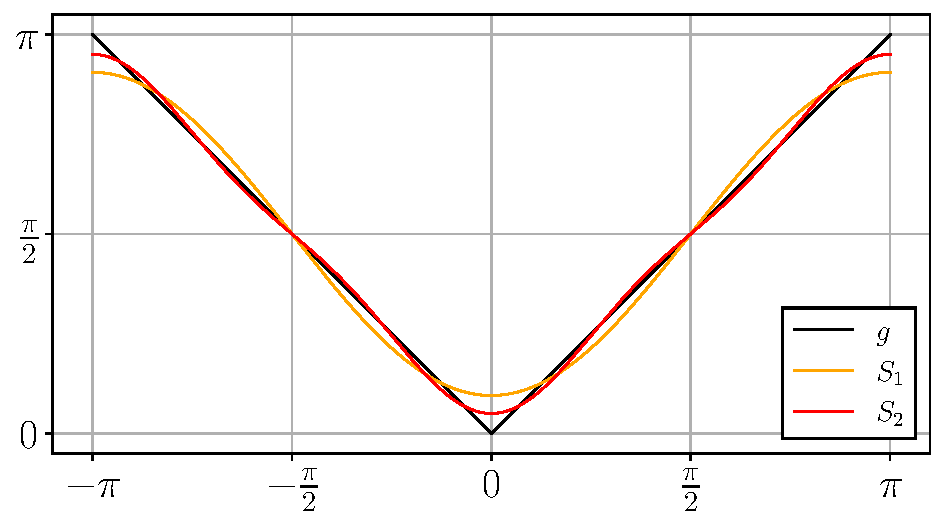
\includegraphics[width=0.8\textwidth]{UA_Section_8_5_Figure_1.pdf}
            \caption{\( g, S_1, \) and \( S_2 \) on \( [-\pi, \pi]\)}
            \label{fig:1}
        \end{figure}
        Notice that
        \[
            \abs{\frac{\cos((2n - 1)x)}{(2n - 1)^2}} \leq \frac{1}{(2n - 1)^2}
        \]
        for each \( n \in \N \) and \( x \in [-\pi, \pi] \). It follows from the Weierstrass M-Test that the series converges uniformly.

        \item For the function \( f \) from Example 8.5.1, notice that \( f \) is not differentiable at \( x = 0 \) or at \( x = \pm \pi \), but satisfies \( f'(x) = 0 \) for all \( x \in (-\pi, 0) \cup (0, \pi) \). The term-by-term differentiated series is
        \[
            \frac{4}{\pi} \sum_{n=0}^{\infty} \cos((2n + 1)x).
        \]
        See \Cref{fig:2} for a graph of \( S_{40} \) and \( S_{80} \) over \( [-\pi, \pi] \).
        \begin{figure}[H]
            \centering
            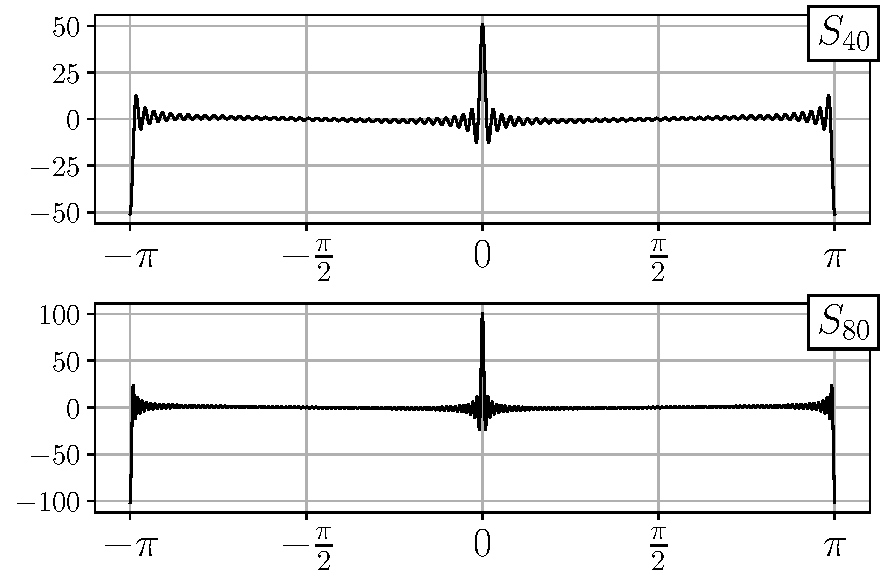
\includegraphics{UA_Section_8_5_Figure_2.pdf}
            \caption{\( S_{40} \) and \( S_{80} \) on \( [-\pi, \pi] \)}
            \label{fig:2}
        \end{figure}
        The series clearly diverges for \( x = 0 \) and \( x = \pm \pi \); this behaviour is reflected in the graph. However, based on the graph we might naively believe that the series is converging to \( f'(x) = 0 \) for all \( x \in (-\pi, 0) \cup (0, \pi) \). In fact, this series converges if and only if \( x = m \pi + \tfrac{\pi}{2} \) for some \( m \in \Z \). If we put the term-by-term differentiated series in the form
        \[
            a_0 + \sum_{n=1}^{\infty} a_n \cos(nx) + b_n \sin(nx),
        \]
        then the coefficients are given by
        \[
            b_n = 0, \quad a_0 = 0, \quand a_n = \begin{cases}
                \frac{4}{\pi} & \text{if } n \text{ is odd}, \\
                0 & \text{if } n \text{ is even},
            \end{cases}
        \]
        which certainly do not allow us to conclude convergence of the term-by-term differentiated series. Furthermore, we cannot use Theorem 6.4.3 since the term-by-term differentiated series does not even converge pointwise, let alone uniformly.

        For the function \( g \) from part (b), notice that \( g \) is not differentiable at \( x = 0 \) or at \( x = \pm \pi \), but satisfies
        \[
            g'(x) = \begin{cases}
                -1 & \text{if } -\pi < x < 0, \\
                1 & \text{if } 0 < x < \pi.
            \end{cases}
        \]
        Notice the similarity to \( f \); indeed, the term-by-term differentiated series is identical to the Fourier series for \( f \):
        \[
            \frac{4}{\pi} \sum_{n=1}^{\infty} \frac{\sin((2n - 1)x)}{2n - 1}.
        \]
        See \Cref{fig:3} for a graph of \( S_4 \) and \( S_{20} \) on \( [-\pi, \pi] \).
        \begin{figure}[H]
            \centering
            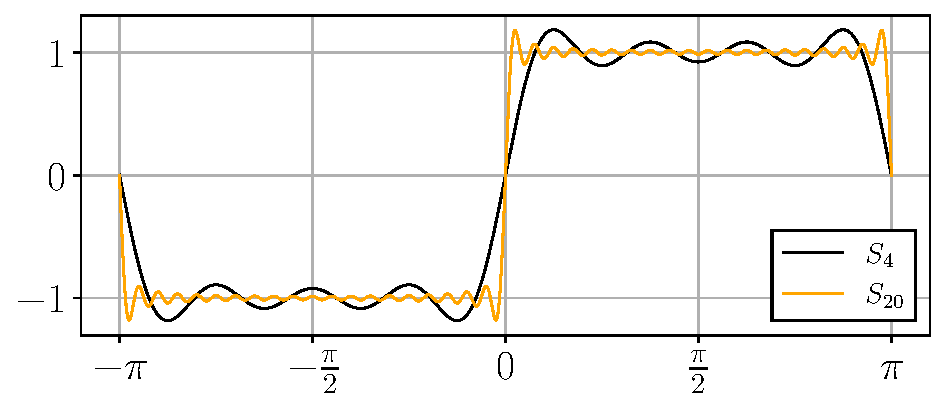
\includegraphics{UA_Section_8_5_Figure_3.pdf}
            \caption{\( S_4 \) and \( S_{20} \) on \( [-\pi, \pi] \)}
            \label{fig:3}
        \end{figure}
        If we put the term-by-term differentiated series in the form
        \[
            a_0 + \sum_{n=1}^{\infty} a_n \cos(nx) + b_n \sin(nx),
        \]
        then the coefficients are given by
        \[
            a_n = 0 \quand b_n = \begin{cases}
                \frac{4}{n \pi} & \text{if } n \text{ is odd}, \\
                0 & \text{if } n \text{ is even},
            \end{cases}
        \]
        which certainly do not allow us to conclude convergence of the term-by-term differentiated series. To use Theorem 6.4.3, we would have to show that the term-by-term differentiated series converges uniformly. At this stage, it is not clear how to do so.
    \end{enumerate}
\end{solution}

\begin{exercise}
\label{ex:5}
    Explain why \( h \) is uniformly continuous on \( \R \).
\end{exercise}

\begin{solution}
    By assumption \( h \) is continuous on the compact set \( [-\pi, \pi] \) and thus, by Theorem 4.4.7, \( h \) is uniformly continuous on \( [-\pi, \pi] \). This is sufficient to show that \( h \) is uniformly continuous on \( \R \), since, by the \( 2 \pi \)-periodicity of \( h \), for any \( x, y \in \R \) there exist integers \( m, n \) such that \( x + 2m \pi \in [-\pi, \pi] \) and \( y + 2n \pi \in [-\pi, \pi] \).
\end{solution}

\begin{exercise}
\label{ex:6}
    Show that \( \abs{\int_a^b h(x) \sin(nx) \, dx} < \epsilon/n \), and use this fact to complete the proof.
\end{exercise}

\begin{solution}
    Let's slightly modify the start of the proof by instead choosing a \( \delta > 0 \) such that \( \abs{h(x) - h(y)} < \tfrac{\epsilon}{2 \pi} \) whenever \( \abs{x - y} < \delta \). For \( x \in [a, b] \), define \( g(x) = h(x) - h \paren{ \tfrac{a + b}{2} } \) and note that \( \abs{g(x)} < \tfrac{\epsilon}{2 \pi} \), since
    \[
        \abs{x - \frac{a + b}{2}} \leq \frac{b - a}{2} = \frac{\pi}{n} < \delta.
    \]
    By \( \frac{2 \pi}{n} \)-periodicity, we have
    \[
        \int_a^b \sin(nx) \, dx = \int_{-\pi/n}^{\pi/n} \sin(nx) \, dx = 0.  
    \]
    Since \( \abs{\sin(nx)} \leq 1 \) for all \( x \in \R \), it follows that
    \begin{multline*}
        \abs{\int_a^b h(x) \sin(nx) \, dx} \leq \abs{h \paren{ \frac{a + b}{2} } \int_a^b \sin(nx) \, dx} + \abs{\int_a^b g(x) \sin(nx) \, dx} \\[2mm]
        \leq \int_a^b \abs{g(x)} \abs{\sin(nx)} \, dx \leq \int_a^b \frac{\epsilon}{2 \pi} \, dx = \frac{\epsilon}{2 \pi} \cdot \frac{2 \pi}{n} = \frac{\epsilon}{n}.
    \end{multline*}
    Now let \( x_0 < x_1 < \cdots < x_n \) be the evenly spaced partition of \( [-\pi, \pi] \) such that each subinterval has length \( \tfrac{2 \pi}{n} \). Then
    \[
        \abs{\int_{-\pi}^{\pi} h(x) \sin(nx) \, dx} = \abs{ \sum_{j=1}^n \int_{x_{j-1}}^{x_j} h(x) \sin(nx) \, dx } \leq \sum_{j=1}^n \abs{ \int_{x_{j-1}}^{x_j} h(x) \sin(nx) \, dx } < \sum_{j=1}^n \frac{\epsilon}{n} = \epsilon.
    \]
    Thus \( \int_{-\pi}^{\pi} h(x) \sin(nx) \, dx \to 0 \) and by repeating this argument with \( \sin \) replaced by \( \cos \), we can show that \( \int_{-\pi}^{\pi} h(x) \cos(nx) \, dx \to 0 \).
\end{solution}

\begin{exercise}
\label{ex:7}
    \begin{enumerate}
        \item First, argue why the integral involving \( q_x(u) \) tends to zero as \( N \to \infty \).

        \item The first integral is a little more subtle because the function \( p_x(u) \) has the \( \sin(u/2) \) term in the denominator. Use the fact that \( f \) is differentiable at \( x \) (and a familiar limit from calculus) to prove that the first integral goes to zero as well.
    \end{enumerate}
\end{exercise}

\begin{solution}
    \begin{enumerate}
        \item The continuity of \( f \) implies the continuity of \( q_x \) and thus by the Riemann-Lebesgue Lemma (Theorem 8.5.2) we have
        \[
            \int_{-\pi}^{\pi} q_x(u) \cos(Nu) \, du \to 0 \text{ as } N \to \infty.
        \]

        \item The continuity of \( p_x \) on \( (-\pi, 0) \cup (0, \pi] \) follows as \( f, \sin, \) and \( \cos \) are continuous everywhere and \( \sin \) is non-zero on \( \paren{ -\tfrac{\pi}{2}, 0 } \cup \left( 0, \tfrac{\pi}{2} \right] \). Strictly speaking, \( p_x \) is not defined at \( u = 0 \). We claim that defining \( p_x(0) = 2 f'(x) \) results in \( p_x \) also being continuous at zero. Observe that for \( u \neq 0 \):
        \[
            \frac{f(u + x) - f(x)}{\sin(u/2)} = 2 \cdot \frac{f(u + x) - f(x)}{u} \cdot \frac{u/2}{\sin(u/2)} \to 2 f'(x) \text{ as } u \to 0,
        \]
        where we have used that \( f \) is differentiable at \( x \) and also that \( \lim_{u \to \infty} \frac{u}{\sin(u)} = 1 \). Thus \( p_x \) is continuous on \( (-\pi, \pi] \) and so we may again use the Riemann-Lebesgue Lemma to conclude that
        \[
            \int_{-\pi}^{\pi} p_x(u) \sin(Nu) \, du \to 0 \text{ as } N \to \infty.
        \]
    \end{enumerate}
\end{solution}

\begin{exercise}
\label{ex:8}
    Prove that if a sequence of real numbers \( (x_n) \) converges, then the arithmetic means
    \[
        y_n = \frac{x_1 + x_2 + x_3 + \cdots + x_n}{n}
    \]
    also converge to the same limit. Give an example to show that it is possible for the sequence of means \( (y_n) \) to converge even if the original sequence \( (x_n) \) does not.
\end{exercise}

\begin{solution}
    Suppose that \( \lim x_n = x \) and let \( \epsilon > 0 \) be given. There exists an \( N_1 \in \N \) such that \( \abs{x_n - x} < \tfrac{\epsilon}{2} \) whenever \( n \geq N_1 \). Choose \( N_2 \in \N \) such that
    \[
        \frac{\abs{x_1 - x} + \cdots + \abs{x_{N_1} - x}}{N_2} < \frac{\epsilon}{2}
    \]
    and suppose that \( n > \max \{ N_1, N_2 \} \). It follows that
    \begin{align*}
        \abs{y_n - x} &= \abs{\frac{x_1 + \cdots + x_{N_1} + x_{N_1 + 1} + \cdots + x_n}{n} - \frac{nx}{n}} \\[2mm]
        &= \abs{ \frac{(x_1 - x) + \cdots + (x_{N_1} - x)}{n} + \frac{(x_{N_1 + 1} - x) + \cdots + (x_n - x)}{n} } \\[2mm]
        &\leq \frac{\abs{x_1 - x} + \cdots + \abs{x_{N_1} - x}}{n} + \frac{\abs{x_{N_1 + 1} - x} + \cdots + \abs{x_n - x}}{n} \\[2mm]
        &< \frac{\epsilon}{2} + \frac{n - N_1}{n} \cdot \frac{\epsilon}{2} \\[2mm]
        &< \epsilon.
    \end{align*}
    Thus \( \lim y_n = x \). For an example where \( (x_n) \) does not converge but \( (y_n) \) does, let \( x_n = (-1)^n \). Then
    \[
        y_n = \begin{cases}
            -\tfrac{1}{n} & \text{if } n \text{ is odd}, \\
            0 & \text{if } n \text{ is even},
        \end{cases}
    \]
    which converges to zero.
\end{solution}

\begin{exercise}
\label{ex:9}
    Use the previous identity to show that
    \[
        \frac{1/2 + D_1(\theta) + D_2(\theta) + \cdots + D_N(\theta)}{N + 1} = \frac{1}{2(N + 1)} \bkt{ \frac{\sin \paren{ (N + 1) \tfrac{\theta}{2} }}{\sin \paren{ \tfrac{\theta}{2} }} }^2.
    \]
\end{exercise}

\begin{solution}
    It will suffice to show that
    \[
        1 + 2 D_1(\theta) + \cdots + 2 D_N(\theta) = \frac{\sin^2 \paren{ (N + 1) \tfrac{\theta}{2} }}{\sin^2 \paren{ \tfrac{\theta}{2} }}.
    \]
    Indeed, using the identities \( \sin(\alpha) \sin(\theta) = \tfrac{1}{2} \paren{ \cos(\alpha - \theta) - \cos(\alpha + \theta) } \) and \( \sin^2(\theta) = \tfrac{1 - \cos(2\theta)}{2} \), we find that
    \begin{align*}
        2 \sum_{k=0}^N D_k(\theta) &= \sum_{k=0}^N \frac{\sin \paren{ \paren{ k + \tfrac{1}{2} } \theta }}{\sin \paren{ \tfrac{\theta}{2} }} \\[2mm]
        &= \frac{1}{\sin^2 \paren{ \tfrac{\theta}{2} }} \sum_{k=0}^N \bkt{ \sin \paren{ \paren{ k + \tfrac{1}{2} } \theta } \sin \paren{ \tfrac{\theta}{2} } } \\[2mm]
        &= \frac{1}{2 \sin^2 \paren{ \tfrac{\theta}{2} }} \sum_{k=0}^N \bkt{ \cos(k\theta) - \cos((k + 1)\theta) } \\[2mm]
        &= \frac{1}{\sin^2 \paren{ \tfrac{\theta}{2} }} \cdot \frac{1 - \cos((N + 1) \theta)}{2} \\[2mm]
        &= \frac{\sin^2 \paren{ (N + 1) \tfrac{\theta}{2} }}{\sin^2 \paren{ \tfrac{\theta}{2} }}.
    \end{align*}
\end{solution}

\begin{exercise}
\label{ex:10}
    \begin{enumerate}
        \item Show that
        \[
            \sigma_N(x) = \frac{1}{\pi} \int_{-\pi}^{\pi} f(u + x) F_N(u) \, du.
        \]

        \item Graph the function \( F_N(u) \) for several values of \( N \). Where is \( F_N \) large, and where is it close to zero? Compare this function to the Dirichlet kernel \( D_N(u) \). Now, prove that \( F_N \to 0 \) uniformly on any set of the form \( \{ u : \abs{u} \geq \delta \} \), where \( \delta > 0 \) is fixed (and \( u \) is restricted to the interval \( (-\pi, \pi] \)).

        \item Prove that \( \int_{-\pi}^{\pi} F_N(u) \, du = \pi \).

        \item To finish the proof of Fejér's Theorem, first choose a \( \delta > 0 \) so that
        \[
            \abs{u} < \delta \quad \text{implies} \quad \abs{f(x + u) - f(x)} < \epsilon.
        \]
        Set up a single integral that represents the difference \( \sigma_N(x) - f(x) \) and divide this integral into sets where \( \abs{u} \leq \delta \) and \( \abs{u} \geq \delta \). Explain why it is possible to make each of these integrals sufficiently small, independently of the choice of \( x \).
    \end{enumerate}
\end{exercise}

\begin{solution}
    \begin{enumerate}
        \item Using the expression for \( S_n(x) \) derived previously in the textbook, we have
        \begin{multline*}
            \sigma_N(x) = \frac{1}{N + 1} \sum_{n=0}^N S_n(x) = \frac{1}{N + 1} \sum_{n=0}^N \frac{1}{\pi} \int_{-\pi}^{\pi} f(u + x) D_n(u) \, du \\[3mm]
            = \frac{1}{\pi} \int_{-\pi}^{\pi} f(u + x) \frac{1}{N + 1} \sum_{n=0}^N D_n(u) \, du = \frac{1}{\pi} \int_{-\pi}^{\pi} f(u + x) F_N(u) \, du.
        \end{multline*}

        \item See \Cref{fig:4} for a graph of \( F_4, F_8, \) and \( F_{12} \) over the interval \( [-\pi, \pi] \).
        \begin{figure}[H]
            \centering
            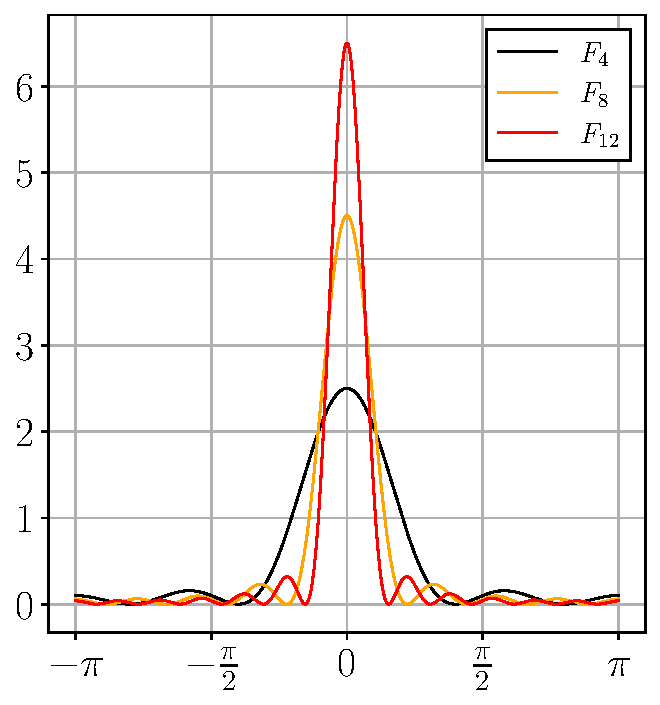
\includegraphics{UA_Section_8_5_Figure_4.pdf}
            \caption{\( F_4, F_8, \) and \( F_{12} \) on \( [-\pi, \pi] \)}
            \label{fig:4}
        \end{figure}
        Like the Dirichlet kernel, the Fejér kernel has a large peak at 0 and decays away from 0; unlike the Dirichlet kernel, the Fejér kernel is non-negative.

        Let \( 0 < \delta < \pi \) be given and set \( A = \{ u \in [-\pi, \pi] : \delta \leq \abs{u} \} \). For any \( u \in A \), observe that \( \sin^2 \paren{ \tfrac{\delta}{2} } \leq \sin^2 \paren{ \tfrac{u}{2} } \). Since \( \delta \in (0, \pi) \), we have \( \sin^2 \paren{ \tfrac{\delta}{2} } > 0 \) and thus
        \[
            \frac{1}{\sin^2 \paren{ \tfrac{u}{2} }} \leq \frac{1}{\sin^2 \paren{ \tfrac{\delta}{2} }}
        \]
        for each \( u \in A \). It follows that
        \[
            \abs{F_N(u)} = \frac{1}{2(N + 1)} \cdot \frac{\sin^2 \paren{ (N + 1) \tfrac{u}{2} }}{\sin^2 \paren{ \tfrac{u}{2} }} \leq \frac{1}{2(N + 1)} \cdot \frac{1}{\sin^2 \paren{ \tfrac{\delta}{2} }}
        \]
        for all \( u \in A \). It is clear from this bound that \( F_N \to 0 \) uniformly on \( A \).

        \item Recalling that \( \int_{-\pi}^{\pi} D_n(u) \, du = \pi \) for any \( n \geq 0 \), we have
        \[
            \int_{-\pi}^{\pi} F_N(u) \, du = \int_{-\pi}^{\pi} \frac{1}{N + 1} \sum_{n=0}^N D_n(u) \, du = \frac{1}{N + 1} \sum_{n=0}^N \int_{-\pi}^{\pi} D_n(u) \, du = \frac{(N + 1) \pi}{N + 1} = \pi.
        \]

        \item By assumption \( f \) is continuous on \( [-\pi, \pi] \) and hence is uniformly continuous here. Thus, for any \( \epsilon > 0 \), we can choose a \( 0 < \delta < \pi \) such that
        \[
            \abs{u} < \delta \quimplies \abs{f(x + u) - f(x)} < \epsilon.
        \]
        For any \( x \in (-\pi, \pi] \) and \( N \in \N \), parts (a) and (c) imply that
        \[
            \sigma_N(x) - f(x) = \frac{1}{\pi} \int_{-\pi}^{\pi} [f(x + u) - f(x)] F_N(u) \, du.
        \]
        Observe that
        \begin{multline*}
            \abs{\frac{1}{\pi} \int_{\abs{u} < \delta} [f(x + u) - f(x)] F_N(u) \, du} \leq \frac{1}{\pi} \int_{\abs{u} < \delta} \abs{f(x + u) - f(x)} F_N(u) \, du \\[2mm]
            < \frac{\epsilon}{\pi} \int_{\abs{u} < \delta} F_N(u) \, du < \frac{\epsilon}{\pi} \int_{-\pi}^{\pi} F_N(u) \, du = \epsilon.
        \end{multline*}
        Let \( M > 0 \) be a bound on \( f \) over \( [-\pi, \pi] \). By part (b), there exists a \( K \in \N \) such that \( F_N(u) \leq \tfrac{\epsilon}{4M} \) for all \( \delta \leq u \leq \pi \) and \( N \geq K \). For such \( N \), observe that
        \begin{multline*}
            \abs{\frac{1}{\pi} \int_{\delta \leq \abs{u} \leq \pi} [f(x + u) - f(x)] F_N(u) \, du} \leq \frac{1}{\pi} \int_{\delta \leq \abs{u} \leq \pi} \abs{f(x + u) - f(x)} F_N(u) \, du \\[2mm]
            \leq \frac{2M \epsilon}{4M \pi} \int_{\delta \leq \abs{u} \leq \pi} \, du < \frac{\epsilon}{2 \pi} \int_{-\pi}^{\pi} \, du = \epsilon.
        \end{multline*}
        It now follows that for any \( x \in (-\pi, \pi] \) and \( N \geq K \), we have
        \begin{multline*}
            \abs{\sigma_N(x) - f(x)} = \abs{ \frac{1}{\pi} \int_{-\pi}^{\pi} [f(x + u) - f(x)] F_N(u) \, du } \\[2mm]
            \leq \abs{\frac{1}{\pi} \int_{\abs{u} < \delta} [f(x + u) - f(x)] F_N(u) \, du} + \abs{\frac{1}{\pi} \int_{\delta \leq \abs{u} \leq \pi} [f(x + u) - f(x)] F_N(u) \, du} < 2 \epsilon.
        \end{multline*}
        We may conclude that \( \sigma_N \to f \) uniformly on \( (-\pi, \pi] \).
    \end{enumerate}
\end{solution}

\begin{exercise}
\label{ex:11}
    \begin{enumerate}
        \item Use the fact that the Taylor series for \( \sin(x) \) and \( \cos(x) \) converge uniformly on any compact set to prove WAT under the added assumption that \( [a, b] \) is \( [0, \pi] \).

        \item Show how the case for an arbitrary interval \( [a, b] \) follows from this one.
    \end{enumerate}
\end{exercise}

\begin{solution}
    \begin{enumerate}
        \item First, let's prove the following result.
        \begin{tcolorbox}
            \textbf{Lemma 1.} Suppose that \( T : \R \to \R \) is a \href{https://en.wikipedia.org/wiki/Trigonometric_polynomial}{trigonometric polynomial}, i.e.\ \( T \) is either constant or of the form
            \[
                T(x) = a_0 + \sum_{n=1}^N a_n \cos(nx) + b_n \sin(nx)
            \]
            for some \( N \in \N \) and some coefficients \( a_n, b_n \in \R \). Let \( [a, b] \) be given. For any \( \epsilon > 0 \), there exists a polynomial \( p \) such that \( \abs{T(x) - p(x)} < \epsilon \) for all \( x \in [a, b] \).
            \tcblower
            \textit{Proof.} If \( T \) is constant the result is clear, so suppose that \( T \) is of the form
            \[
                T(x) = a_0 + \sum_{n=1}^N a_n \cos(nx) + b_n \sin(nx)
            \]
            for some \( N \in \N \) and some coefficients \( a_n, b_n \in \R \). Let \( 1 \leq n \leq N \) be given. Because the Taylor series for \( \cos(nx) \) converges uniformly on \( [a, b] \), there exists a polynomial \( p_n \) (some partial sum of the Taylor series) such that
            \[
                \abs{\cos(nx) - p_n(x)} < \frac{\epsilon}{2N(1 + \abs{a_n})}
            \]
            for each \( x \in [a, b] \). Similarly, there exists a polynomial \( q_n \) such that
            \[
                \abs{\sin(nx) - q_n(x)} < \frac{\epsilon}{2N(1 + \abs{b_n})}
            \]
            for each \( x \in [a, b] \). Let \( p \) be the polynomial given by \( p(x) = a_0 + \sum_{n=1}^N a_n p_n(x) + b_n q_n(x) \). Then for any \( x \in [a, b] \), we have
            \begin{align*}
                \abs{T(x) - p(x)} &= \abs{ \sum_{n=1}^N a_n (\cos(nx) - p_n(x)) + b_n (\sin(nx) - q_n(x)) } \\[2mm]
                &\leq \sum_{n=1}^N \abs{a_n} \abs{\cos(nx) - p_n(x)} + \abs{b_n} \abs{\sin(nx) - q_n(x)} \\[2mm]
                &< \sum_{n=1}^N \frac{\epsilon \abs{a_n}}{2N(1 + \abs{a_n})} + \frac{\epsilon \abs{b_n}}{2N(1 + \abs{b_n})} \\[2mm]
                &< \sum_{n=1}^N \frac{\epsilon}{N} \\[2mm]
                &= \epsilon. \tag*{\qed}
            \end{align*}
        \end{tcolorbox}

        Now let \( f : [0, \pi] \to \R \) be continuous and let \( \epsilon > 0 \) be given. By Fejér's Theorem (Theorem 8.5.4), \( \sigma_N \to f \) uniformly on \( [0, \pi] \) and thus there exists an \( M \in \N \) such that \( \abs{\sigma_M(x) - f(x)} < \tfrac{\epsilon}{2} \) for all \( x \in [0, \pi] \). Notice that \( \sigma_M \) is a trigonometric polynomial; it follows from Lemma 1 that there exists a polynomial \( p \) such that \( \abs{\sigma_M(x) - p(x)} < \tfrac{\epsilon}{2} \) for all \( x \in [0, \pi] \). Thus
        \[
            \abs{f(x) - p(x)} \leq \abs{\sigma_M(x) - f(x)} + \abs{\sigma_M(x) - p(x)} < \epsilon
        \]
        for any \( x \in [0, \pi] \).

        \item Let \( f : [a, b] \to \R \) be continuous and define \( g : [0, \pi] \to \R \) by \( g(x) = f \paren{ \frac{b - a}{\pi} x + a } \); notice that \( g \) is continuous. Let \( \epsilon > 0 \) be given. By part (a), there exists a polynomial \( q \) such that \( \abs{g(x) - q(x)} < \epsilon \) for each \( x \in [0, \pi] \). Define \( p \) by \( p(x) = q \paren{ \frac{\pi(x - a)}{b - a} } \) and notice that \( p \) is a polynomial. For any \( x \in [a, b] \) we have \( \tfrac{\pi (x - a)}{b - a} \in [0, \pi] \) and thus
        \[
            \abs{ g \paren{ \frac{\pi (x - a)}{b - a} } - q \paren{ \frac{\pi(x - a)}{b - a} }} = \abs{f(x) - p(x)} < \epsilon.
        \]
    \end{enumerate}
\end{solution}

\noindent \hrulefill

\noindent \hypertarget{ua}{\textcolor{blue}{[UA]} Abbott, S. (2015) \textit{Understanding Analysis.} 2\ts{nd} edition.}

\end{document}